% Boxes of text with sub- and superscripts in inline math, in nodes of a
% set text width, saved in a box: the formulas are rigid, so the size of
% the paragraphs stays known, and so do the picture's anchors.
\documentclass{article}
\usepackage{tikz}
\usetikzlibrary{positioning}
\newcommand{\entry}[4]{%
  \node[below=1mm of #1, text width=#3, draw=blue!20, fill=blue!10] (#2)
    {\small #4};}
\begin{document}
\newsavebox{\sketch}
\sbox{\sketch}{\parbox{0.3\textwidth}{%
  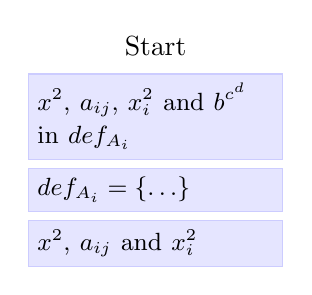
\begin{tikzpicture}
    \node (a) {Start};
    \entry{a}{b}{3cm}{$x^2$, $a_{ij}$, $x_i^2$ and $b^{c^d}$ in $def_{A_i}$}
    \entry{b}{c}{3cm}{$def_{A_i}=\{\dots\}$}
    \entry{c}{d}{3cm}{$x^2$, $a_{ij}$ and $x_i^2$}
  \end{tikzpicture}}}
\colorlet{mixed}{gray!50!blue}
\begin{tikzpicture}
  \node[fill=mixed] (s) {\usebox{\sketch}};
  \node[right=1cm of s, draw] {$x^2$};
\end{tikzpicture}
\gdef\SatexReachedEnd{}
\end{document}
